\documentclass[11pt,letterpaper]{article}
\usepackage[margin=2cm]{geometry}
\usepackage{amsmath,amssymb,graphicx,xcolor,booktabs,tabularx,enumitem,titlesec,fancyhdr,array,longtable,caption}
\usepackage{tikz}
\usetikzlibrary{arrows.meta,positioning,shapes.geometric,calc}
\usepackage[hidelinks]{hyperref}
\usepackage{helvet}\renewcommand{\familydefault}{\sfdefault}
\usepackage{microtype}
\titleformat{\section}{\Large\bfseries\color{blue!50!black}}{\thesection}{0.6em}{}
\titleformat{\subsection}{\large\bfseries}{\thesubsection}{0.6em}{}
\titleformat{\subsubsection}{\normalsize\bfseries\color{blue!40!black}}{}{0em}{}
\setlength{\headheight}{14pt}
\pagestyle{fancy}\fancyhf{}\lhead{sPHENIX Self-Paced Course}\rhead{Module 1: Physics program}\cfoot{\thepage}
\setlist{itemsep=1pt,topsep=3pt}
\setlength{\emergencystretch}{3em}
\setlength{\parskip}{3pt}
\newcommand{\conceptbox}[2]{\par\medskip\noindent\fcolorbox{blue!50!black}{blue!5}{\begin{minipage}{0.96\linewidth}\textbf{#1}\par\smallskip #2\end{minipage}}\par\medskip}
\newcommand{\connectbox}[1]{\par\medskip\noindent\fcolorbox{green!40!black}{green!6}{\begin{minipage}{0.96\linewidth}\textbf{Connect to your analysis.}\par\smallskip #1\end{minipage}}\par\medskip}
\newcommand{\pitfallbox}[1]{\par\medskip\noindent\fcolorbox{red!50!black}{red!4}{\begin{minipage}{0.96\linewidth}\textbf{Pitfalls.}\par\smallskip #1\end{minipage}}\par\medskip}
\newcommand{\checksbox}[1]{\par\medskip\noindent\fcolorbox{orange!60!black}{orange!6}{\begin{minipage}{0.96\linewidth}\textbf{Checks.}\par\smallskip #1\end{minipage}}\par\medskip}
\newcommand{\goal}[1]{\noindent\textbf{Goal.} #1\par}
\newcommand{\sqs}{\sqrt{s_{_{NN}}}}
\newcommand{\pT}{p_{\mathrm{T}}}
\newcommand{\RAA}{R_{AA}}
\begin{document}
\begin{center}
{\LARGE\bfseries sPHENIX Self-Paced Course}\\[4pt]
{\Large Module 1: The sPHENIX physics program:\\ QGP, jets, heavy flavour, cold QCD and spin}\\[8pt]
Prepared for P.\,D.\ Lewis (Ohio University) \quad November 2026\\[2pt]
\small Self-contained study text based on the Summer-2026 sPHENIX School (BNL, July 2026), public sPHENIX papers and standard textbook physics
\end{center}

\tableofcontents
\newpage

\section*{How to use this module}
\addcontentsline{toc}{section}{How to use this module}
This module is self-contained. You do not need the school slides, recordings or papers to follow it: every concept is
built up here from first principles to sPHENIX practice, with the reasoning, short derivations and worked numbers.
The school talks listed below are the \emph{sources} that the text paraphrases; they are cited as [S\#\#] so that you
can trace a statement back if you ever want to. Read the module straight through once. Then reread it and answer the
self-test questions (Section~\ref{sec:selftest}) before looking at the answers in Appendix~\ref{app:answers}.
The hands-on exercises are optional; nothing in the text depends on doing them.

\subsection*{Learning objectives}
After this module you should be able to:
\begin{enumerate}[label=O\arabic*.]
\item State what the quark--gluon plasma (QGP) is, why it exists in QCD, and why RHIC and the LHC are complementary.
\item Use the basic kinematic variables ($\pT$, $y$, $\eta$, $\sqs$, invariant cross section) fluently, with numbers.
\item Explain the Bjorken energy density, collective flow ($v_n$, eccentricity, cumulants) and what the Bulk topical group measures.
\item Derive the key scalings of jet quenching (broadening $\hat q L$, formation time, $\omega_c=\hat qL^2$, $\Delta E\propto L^2$, colour coherence) and connect them to $\RAA$, dijets and substructure.
\item Explain why heavy quarks and quarkonia probe the QGP, and what the Heavy Flavor topical group needs from tracking.
\item Explain transverse single-spin asymmetries, the Sivers and Collins mechanisms, twist-3 correlators, and the cold-QCD channels in sPHENIX.
\item Summarise the history from PHENIX to sPHENIX and the organisation into topical groups and paper preparation groups.
\item Place neutral-meson measurements ($\pi^0$, $\eta$ cross sections, $\RAA$/$R_{CP}$, $A_N$, $v_2$) in the whole programme.
\end{enumerate}

\subsection*{Prerequisites, time and sources}
\textbf{Prerequisites:} none within the course (this is Module 1). Undergraduate special relativity and quantum mechanics.
\textbf{Estimated time:} 9--10 hours (reading 6 h, self-test 2 h, optional exercises 1--2 h).

\noindent\textbf{School talks used as sources} (all ``sPHENIX School 2026'', BNL, July--August 2026):
\begin{itemize}
\item {[S01]} J.\ Huang, M.\ Connors, ``Welcome to sPHENIX school and sPHENIX Overview''.
\item {[S02]} D.\ Morrison, ``sPHENIX History''.
\item {[S03]} Y.\ Mehtar-Tani, ``sPHENIX Theory Overview: exploring QGP dynamics with jets''.
\item {[S04]} G.\ Nukazuka, M.\ Sarsour, ``Cold QCD TG Analysis Opportunities''.
\item {[S05]} M.\ Mitrankova, R.\ Belmont, ``Bulk TG Analysis Opportunities''.
\item {[S06]} A.\ Frawley, C.\ Dean, G.\ Ottino, M.\ Rosati, ``Heavy Flavor TG Analysis Opportunities''.
\item {[S07]} J.\ Putschke, Y.\ Go, ``Jet Structure TG Analysis Opportunities''.
\item {[S44]} G.\ Nukazuka, ``Cold QCD Lecture Series announcement''; {[S50]} M.\ Cerutti, ``Cold-QCD lecture (workfest)''.
\item Supporting: {[S08]} J.\ Haggerty (sPHENIX timeline), {[S48]} K.\ Hock (polarized protons at RHIC).
\end{itemize}
\textbf{Public readings} (optional): the first two sPHENIX Au+Au papers on charged-hadron multiplicity
\cite{bulk1} and transverse energy \cite{bulk2}; the first $p$+$p$ papers on dijet imbalance \cite{dijet} and isolated
photons \cite{isogamma}; the sPHENIX proposal \cite{proposal}; overview talks \cite{nouicer,roland}.

\section{Why sPHENIX exists: QCD, the QGP and hard probes}\label{sec:why}
\goal{Understand the physics question that sPHENIX was built to answer, starting from the basic properties of QCD.}

\subsection{QCD in one page}
Quantum chromodynamics (QCD) is the theory of quarks and gluons. Quarks carry one of three ``colour'' charges; gluons
carry colour themselves and therefore interact with each other. That self-interaction is the origin of the two
properties that dominate everything in this course.

\textbf{Asymptotic freedom.} The strong coupling decreases with the momentum transfer $Q$ of a process. At one loop
\begin{equation}
\alpha_s(Q^2)=\frac{12\pi}{(33-2n_f)\,\ln(Q^2/\Lambda_{\rm QCD}^2)},\qquad \Lambda_{\rm QCD}\approx 0.2\ \mathrm{GeV},
\label{eq:alphas}
\end{equation}
with $n_f$ active quark flavours. For $Q=10$ GeV and $n_f=5$ this gives $\alpha_s\approx 12\pi/(23\ln 2500)\approx 0.21$;
for $Q=1$ GeV it gives $\approx 0.5$. Hard processes (large $Q$) are therefore calculable in perturbation theory (pQCD).

\textbf{Confinement.} At low $Q$ (large distances) the coupling is large; isolated colour charges are never observed.
Quarks and gluons appear only inside hadrons. The energy stored in the colour field between separating charges grows
roughly linearly with distance, until it is cheaper to create a new quark--antiquark pair; this is \emph{hadronization}.

\textbf{Deconfinement.} Lattice QCD (numerical QCD on a space-time grid) shows that at temperatures above
$T_c\approx 155$ MeV (about $2\times10^{12}$ K) hadronic matter turns into a medium where colour is screened over
distances of the order of the inter-particle spacing. This medium is the quark--gluon plasma. The transition at zero net
baryon density is a smooth crossover, not a sharp phase transition. The universe passed through this state a few
microseconds after the Big Bang. The critical energy density is of order 1 GeV/fm$^3$, compared with about 0.15
GeV/fm$^3$ in ordinary nuclear matter and about 0.5 GeV/fm$^3$ inside a proton [S05].

\subsection{What RHIC learned, and the open question}
RHIC began colliding nuclei in 2000 [S02]. Two discoveries defined the field. First, the produced matter flows
collectively, and relativistic viscous hydrodynamics describes the flow only if the shear viscosity to entropy
density ratio is very small, $\eta/s\approx0.1$, close to the conjectured quantum lower bound $1/4\pi\approx0.08$.
The QGP behaves as an almost perfect liquid, far less viscous (in this dimensionless sense) than water or helium [S03].
Second, high-$\pT$ hadrons are strongly suppressed in central Au+Au collisions relative to scaled $p$+$p$ collisions;
PHENIX first reported this with charged hadrons and $\pi^0$s \cite{phenixsupp,phenixwp}. This is \emph{jet quenching}.

These discoveries raise a deeper question. A perfect liquid is a strongly coupled system with no well-defined
quasi-particles; but at very short distances asymptotic freedom says the QGP must look like weakly coupled quarks and
gluons. \emph{How does the liquid-like behaviour emerge from QCD as a function of the resolution scale?} [S03]
Answering this needs probes that resolve the medium at different length scales: jets of different energies and
radii, heavy quarks of different masses, and quarkonium states of different sizes.

\subsection{The sPHENIX answer}
The 2015 US Nuclear Physics Long Range Plan stated that a central goal of RHIC and the LHC is to probe the QGP at
shorter and shorter length scales, and that a state-of-the-art jet detector at RHIC---sPHENIX---is essential for that;
the 2023 plan asked to complete the sPHENIX programme as part of concluding the RHIC science mission [S01].
The design follows directly from the physics [S01]:
\begin{itemize}
\item \textbf{Central calorimetry} (EMCal + inner and outer HCal, $|\eta|<1.1$, full azimuth) for full jet
reconstruction and for photons and electrons.
\item \textbf{Central tracking} (MVTX, INTT, TPC, TPOT) in a 1.4 T solenoid for heavy-flavour tagging, quarkonia and jet
substructure with charged particles.
\item \textbf{Forward detectors} (MBD, sEPD, ZDC) for triggering and event characterisation (vertex, centrality, event plane).
\item \textbf{A high-rate DAQ}, including streaming readout of the trackers, to record very large minimum-bias samples.
\end{itemize}

\conceptbox{Why RHIC when the LHC exists?}{The LHC reaches much higher energy, so hard probes are more abundant there.
RHIC is complementary for three reasons. (1) The QGP at RHIC is produced closer to $T_c$, where the medium is expected
to be most strongly coupled; comparing RHIC and LHC tests the temperature dependence of transport properties.
(2) At RHIC the underlying event is smaller and jets of a given $\pT$ come from a different mix of quarks and gluons
and a different region of the parton distributions. (3) RHIC uniquely provides polarized proton beams, so the same
detector can run a spin programme. sPHENIX brings LHC-style calorimetric jet reconstruction to RHIC energies [S01,S03].}

\checksbox{You understand this section if you can explain, without notes: (a) why pQCD works for jets but not for
the bulk; (b) what ``almost perfect liquid'' means in terms of $\eta/s$; (c) why a short-distance probe is needed to
answer the emergence question.}

\section{Kinematics toolkit}\label{sec:kin}
\goal{Be fluent with the variables every sPHENIX analysis uses, with numbers you can check in your head.}

\subsection{Variables}
Take the beam along $z$. For a particle with energy $E$ and momentum $\vec p$:
\begin{align}
\pT&=\sqrt{p_x^2+p_y^2},\qquad m_{\mathrm T}=\sqrt{\pT^2+m^2},\\
y&=\tfrac12\ln\frac{E+p_z}{E-p_z},\qquad \eta=-\ln\tan(\theta/2)=\tfrac12\ln\frac{|\vec p|+p_z}{|\vec p|-p_z}.
\end{align}
Rapidity $y$ is additive under boosts along $z$: a boost changes every $y$ by the same constant, so shapes of $dN/dy$
are boost invariant. Pseudorapidity $\eta$ depends only on the polar angle, which is what a detector measures; $y\to\eta$ when $\pT\gg m$.
Useful relations: $E=m_{\mathrm T}\cosh y$, $p_z=m_{\mathrm T}\sinh y$.

\textbf{Worked numbers.} The central barrel covers $|\eta|<1.1$, i.e.\ polar angles $36.8^\circ<\theta<143.2^\circ$.
The sEPD covers $2.0<|\eta|<4.9$, i.e.\ $15.4^\circ$ down to $0.85^\circ$ from the beam. The MBD covers about
$3.5<|\eta|<4.6$, i.e.\ $3.4^\circ$ to $1.1^\circ$ [S08]. A 100 GeV/nucleon Au beam has
$y_{\rm beam}=\cosh^{-1}(E/m_N)\approx\ln(\sqs/m_N)=\ln(200/0.938)\approx5.36$.

\subsection{Centre-of-mass energy and the invariant cross section}
For symmetric collisions $\sqrt{s}=2E_{\rm beam}$. For nuclei one quotes the energy per nucleon pair, $\sqs$; RHIC
Au+Au, O+O and $p$+$p$ in sPHENIX were all at $\sqs=200$ GeV. The Lorentz-invariant differential cross section is
\begin{equation}
E\frac{d^3\sigma}{dp^3}=\frac{1}{2\pi\pT}\frac{d^2\sigma}{d\pT\,dy}.
\label{eq:invxs}
\end{equation}
The factor $1/(2\pi\pT)$ comes from $d^3p=\pT\,d\pT\,d\phi\,dp_z$ and $dp_z/E=dy$, integrated over $\phi$.
In an experiment, with $N$ counts in a bin, integrated luminosity $\mathcal L$, efficiency $\varepsilon$, acceptance $A$ and
branching ratio $B$,
\begin{equation}
E\frac{d^3\sigma}{dp^3}=\frac{1}{2\pi\pT}\,\frac{N}{\mathcal L\,\varepsilon A\,B\,\Delta\pT\,\Delta y}.
\end{equation}
For heavy ions the per-event invariant yield replaces $\sigma/\mathcal L$ by $N/N_{\rm evt}$.

\subsection{Scaling variable $x_T$}
In a $2\to2$ hard scattering at $y=0$ a hadron of transverse momentum $\pT$ probes parton momentum fractions of order
$x_T=2\pT/\sqrt{s}$. A 10 GeV $\pi^0$ at RHIC has $x_T=0.1$; the same $x_T$ at the LHC (5.02 TeV) corresponds to
$\pT\approx250$ GeV. This is one reason RHIC probes a different quark/gluon mix: at fixed $\pT$, RHIC is at larger $x$,
where quarks matter more.

\connectbox{Your $p$+$p$ $\pi^0$/$\eta$ cross section is exactly Eq.~(\ref{eq:invxs}) with $B=B(\pi^0\to\gamma\gamma)$ or
$B(\eta\to\gamma\gamma)$, $\mathcal L$ from the GL1 scalers, $\varepsilon A$ from PYTHIA8 with EMCal smearing, and the
trigger efficiency folded in. The $|y|$ window of the pair (not $|\eta|$ of each photon) defines $\Delta y$. Always check
that your $\varepsilon A$ is defined with the same $\Delta y$ and the same $\pT$ binning as the raw yield.}

\section{The life of a heavy-ion collision and the Bulk programme}\label{sec:bulk}
\goal{Know the stages of a heavy-ion collision, how its global properties (energy density, multiplicity, flow) are
measured, and which measurements the Bulk topical group (TG) pursues in sPHENIX.}

\subsection{Stages of the collision}
Figure~\ref{fig:timeline} is the ``standard model'' of a heavy-ion collision [S05]. Two Lorentz-contracted nuclei
(at 100 GeV/nucleon the contraction factor is $\gamma\approx107$, so a gold nucleus of radius 7 fm is about 0.13 fm thick)
pass through each other. Hard scatterings (jets, heavy quarks, prompt photons) happen first, within $\sim1/\pT$.
A dense, initially far-from-equilibrium gluon system (often called the glasma) forms. Within about 1 fm/$c$ it becomes
well described by hydrodynamics; modern theory calls this \emph{hydrodynamization} rather than thermalization,
because hydrodynamics can work before full local equilibrium [S05]. The QGP expands and cools for a few fm/$c$,
hadronizes near $T_c$, and the hadrons stop changing species (chemical freeze-out) and then stop interacting (kinetic
freeze-out). The detector sees only the final hadrons, leptons and photons.

\begin{figure}[h]\centering
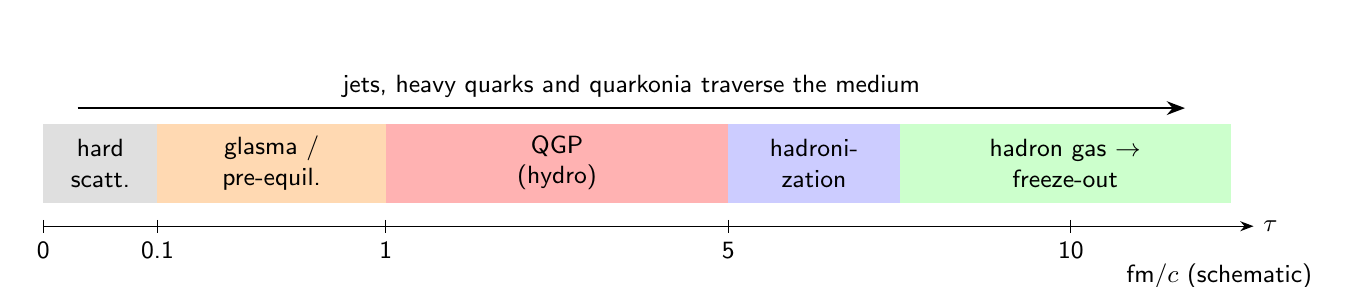
\begin{tikzpicture}[x=1.45cm,y=1cm,font=\small]
\draw[-{Stealth}] (0,0)--(10.6,0) node[right]{$\tau$};
\foreach \x/\l in {0/0,1/0.1,3/1,6/5,9/10}{\draw (\x,0.08)--(\x,-0.08) node[below]{\l};}
\node[below] at (10.3,-0.35) {fm/$c$ (schematic)};
\fill[gray!25] (0,0.3) rectangle (1,1.3); \node[align=center] at (0.5,0.8){hard\\scatt.};
\fill[orange!30] (1,0.3) rectangle (3,1.3); \node[align=center] at (2,0.8){glasma /\\pre-equil.};
\fill[red!30] (3,0.3) rectangle (6,1.3); \node[align=center] at (4.5,0.8){QGP\\(hydro)};
\fill[blue!20] (6,0.3) rectangle (7.5,1.3); \node[align=center] at (6.75,0.8){hadroni-\\zation};
\fill[green!20] (7.5,0.3) rectangle (10.4,1.3); \node[align=center] at (8.95,0.8){hadron gas $\to$\\freeze-out};
\draw[thick,-{Stealth}] (0.3,1.5)--(10,1.5) node[midway,above]{jets, heavy quarks and quarkonia traverse the medium};
\end{tikzpicture}
\caption{Schematic time line of a central heavy-ion collision at RHIC (not to scale; times are order-of-magnitude).}
\label{fig:timeline}\end{figure}

\subsection{Bjorken picture and energy density}
Two pictures of stopping compete [S05]. In Landau's picture the nuclei stop each other and $dN/dy$ is roughly
Gaussian. In Bjorken's picture the nuclei pass through each other and leave a boost-invariant region of produced
matter; $dN/dy$ is flat near $y=0$ \cite{bjorken}. RHIC data (PHOBOS, BRAHMS) show that the Bjorken picture is the
right starting point at 200 GeV [S05].

\textbf{Derivation.} In the boost-invariant picture, the matter at rapidity $y$ is at $z=t\tanh y$, i.e.\ at proper
time $\tau=\sqrt{t^2-z^2}$ a slice $dy$ occupies a longitudinal length $dz=\tau\,dy$ (at $y\approx0$). If the
transverse overlap area is $A_T$, the volume of the slice is $A_T\tau\,dy$ and the energy in it is $dE_T$. Hence
\begin{equation}
\varepsilon_{\rm Bj}(\tau)=\frac{1}{\tau A_T}\frac{dE_T}{dy},\qquad E_T=\sum_i E_i\sin\theta_i .
\label{eq:bj}
\end{equation}
\textbf{Worked example (round numbers).} For a central Au+Au collision take $A_T=\pi R^2$ with $R=1.18A^{1/3}$ fm
$=6.9$ fm, so $A_T\approx148$ fm$^2$. With $dE_T/d\eta\approx600$ GeV and a Jacobian $dE_T/dy\approx1.25\,dE_T/d\eta$,
at $\tau=1$ fm/$c$ one gets $\varepsilon\approx(1.25\times600)/148\approx5$ GeV/fm$^3$, several times the critical
value. These are illustrative round numbers of the size found by the RHIC experiments. Because $A_T$ is fairly
well determined from centrality (Glauber modelling, Module 2) but $\tau$ is model dependent, experiments often quote
the product $\varepsilon\tau$ [S05].

\subsection{How sPHENIX measured $dE_T/d\eta$ and $dN_{ch}/d\eta$}
The first two sPHENIX physics papers came from the Bulk TG [S05]:
\begin{itemize}
\item \textbf{Transverse energy} \cite{bulk2}. Each calorimeter layer (EMCal, inner HCal, outer HCal) measures
$\sum E_{T,\rm tower}(\eta)$. A correction factor $C(\eta)=\sum E_{T,\rm tower}/\sum E_{T,\rm particle}$, built from
HIJING events reweighted to match measured identified-particle spectra, converts the tower sum into the true
$dE_T/d\eta$. The EMCal sees the largest fraction of the total energy, the outer HCal much less, and the inner HCal
(mostly aluminium) only a small fraction. Agreement between the EMCal-based and HCal-based results is a strong internal check.
\item \textbf{Charged-hadron multiplicity} \cite{bulk1}. Using Run-2024 Au+Au data taken with the magnet off (straight tracks), charged hadrons were counted as pairs of clusters in the inner and outer INTT layers. $dN_{ch}/d\eta$ was obtained with two very different methods
with different systematics; their agreement shows systematic control. The result agrees with earlier PHOBOS data, and
the centrality dependence is not a simple scaling with the number of participants.
\end{itemize}
\textbf{Two-component model.} A common parametrization is
$dN_{ch}/d\eta=n_{pp}\left[(1-x)\,\frac{N_{\rm part}}{2}+x\,N_{\rm coll}\right]$, where $N_{\rm part}$ (participants) and
$N_{\rm coll}$ (binary collisions) come from Glauber modelling and $x$ is the ``hard'' fraction. As a toy check, with
$n_{pp}=2.4$, $x=0.13$, $N_{\rm part}=350$ and $N_{\rm coll}=1050$ one gets about 690. The model is not the end of the
story; participant-quark scaling is an alternative and the question is not settled [S05].

\subsection{Collective flow}
The overlap region of a non-central collision is almond shaped. Pressure gradients are larger along the short axis,
so more particles are pushed in that direction. Expanding the azimuthal distribution in a Fourier series around the
symmetry planes $\Psi_n$,
\begin{equation}
\frac{dN}{d\phi}\propto1+\sum_{n=1}^{\infty}2v_n\cos[n(\phi-\Psi_n)],\qquad v_n=\langle\cos[n(\phi-\Psi_n)]\rangle .
\label{eq:flow}
\end{equation}
The initial shape is quantified by the eccentricities
$\varepsilon_n=\sqrt{\langle r^n\cos n\phi\rangle^2+\langle r^n\sin n\phi\rangle^2}/\langle r^n\rangle$, averaged over the
initial energy (or nucleon) density [S05]. Hydrodynamics converts shape into momentum anisotropy; to a good
approximation $v_2\approx\kappa_2\varepsilon_2$ and $v_3\approx\kappa_3\varepsilon_3$, where the response coefficients
$\kappa_n$ decrease with viscosity and with $n$ (viscosity damps fine structure first). This is how flow constrains $\eta/s$.

\textbf{Centrality dependence of $v_2$.} $v_2$ rises from central to mid-central collisions and falls again in
peripheral ones. Two effects compete: more peripheral means larger $\varepsilon_2$ (higher $v_2$), but also a smaller
system with fewer interactions and less time to build flow (lower $v_2$) [S05].

\textbf{Fluctuations and odd harmonics.} Nuclei are made of nucleons at random positions, so the initial state is
lumpy. Event-by-event fluctuations give non-zero odd eccentricities ($\varepsilon_3$, triangular flow $v_3$) and
symmetry planes $\Psi_n$ that differ between harmonics \cite{alverroland}. Measured $v_3$ is indeed non-zero [S05].

\textbf{Cumulants.} Multi-particle correlations measure moments of the $v_n$ distribution and suppress non-flow
(few-particle correlations such as jets and decays). If $v_2$ fluctuates around $\bar v$ with small variance $\sigma^2$,
\begin{align}
v_2\{2\}^2&=\langle v_2^2\rangle=\bar v^2+\sigma^2,\\
v_2\{4\}^4&=2\langle v_2^2\rangle^2-\langle v_2^4\rangle\approx(\bar v^2-\sigma^2)^2,
\end{align}
so $v_2\{2\}\approx\sqrt{\bar v^2+\sigma^2}$ and $v_2\{4\}\approx v_2\{6\}\approx v_2\{8\}\approx\sqrt{\bar v^2-\sigma^2}$.
Small deviations between $v_2\{4\},v_2\{6\},v_2\{8\}$ measure the non-Gaussian shape of the fluctuations; the ratio
$\sigma_{v_2}/\langle v_2\rangle$ tests initial-state models. In very central collisions the small-variance
approximation breaks down; in peripheral ones the hydro response becomes non-linear [S05]. With minimum-bias Au+Au samples far larger than those available to PHENIX, sPHENIX can push these measurements to high precision and to higher harmonics and
correlations between harmonics (normalized symmetric cumulants) [S05].

\subsection{Small systems and the ridge}
In two-particle correlations versus $\Delta\eta$ and $\Delta\phi$, a near-side structure extended over many units of
$\Delta\eta$ (the \emph{ridge}) is a signature of collective flow; it was seen first in Au+Au at RHIC and later in
high-multiplicity $p$+$p$ at the LHC [S05]. Whether a ridge exists in $p$+$p$ at RHIC is an open question that the
large sPHENIX minimum-bias and high-multiplicity samples can address. Collision geometry differs between small systems:
d+Au has a large intrinsic $\varepsilon_2$ from the two-nucleon projectile, while O+O acquires $\varepsilon_3$ only
through fluctuations. The sPHENIX O+O data are therefore valuable for separating geometry from response [S05].

\subsection{How it is done in sPHENIX}
\begin{itemize}
\item Acceptance: the central barrel ($|\eta|<1.1$) for particles of interest, and the sEPD ($2.0<|\eta|<4.9$) or MBD for
symmetry planes. A large rapidity gap between the two suppresses non-flow [S05].
\item Event-plane method: $Q$-vectors $Q_n=\sum_j w_j e^{in\phi_j}$ from sEPD tiles give $\Psi_n$; the observed
$v_n^{\rm obs}=\langle\cos n(\phi-\Psi_n)\rangle$ is divided by the event-plane resolution (Module 2). In coresoftware the
module is \texttt{EventPlaneReco} (package \texttt{eventplaneinfo}); centrality comes from \texttt{CentralityReco}.
\item Neutral mesons: $\pi^0$ $v_2$ uses the same EMCal diphoton pairs as your $\RAA$ analysis, binned in
$\phi-\Psi_2$; the signal yield per bin is fitted and the modulation extracted. It is an EMCal performance benchmark
against PHENIX measurements [S05].
\item Multiplicity in O+O: ongoing analyses use silicon tracking (see Module 10 case studies [S25,S26]).
\end{itemize}

\checksbox{(1) A flow analysis must show that $v_n$ does not depend on the choice of event-plane detector once
resolution-corrected (north vs south sEPD, MBD vs sEPD). (2) $v_2\{4\}<v_2\{2\}$ is expected; the opposite usually
signals a bug or non-flow. (3) $dE_T/d\eta$ from the EMCal and from the HCal must agree within systematic uncertainties.}

\pitfallbox{Confusing $\eta$ and $y$ when converting $dE_T/d\eta$ to $dE_T/dy$ (the Jacobian depends on the particle
mix). Forgetting that $v_n$ from a single event plane mixes $\bar v$ and fluctuations differently from cumulants.
Ignoring non-flow in peripheral and small systems.}

\section{Jets as probes of the QGP: theory of jet quenching}\label{sec:jets}
\goal{Understand, with simple derivations, why and how energetic partons lose energy in the QGP, and what each class of
jet observable is sensitive to. This is the core physics motivation of sPHENIX [S03].}

\subsection{Jets in vacuum: a calibrated probe}
A jet is the collimated spray of hadrons produced when an energetic quark or gluon showers and hadronizes. After five
decades of work---from the discovery of the gluon in three-jet events at DESY in 1979 to the Higgs discovery---jet
cross sections and shapes in vacuum are predicted with few-percent precision [S03]. In $p$+$p$ collisions the
cross section factorizes:
\begin{equation}
d\sigma^{pp\to h X}=\sum_{a,b,c}f_a(x_1,\mu^2)\otimes f_b(x_2,\mu^2)\otimes d\hat\sigma_{ab\to cX}(\mu^2)\otimes D_{c\to h}(z,\mu^2),
\label{eq:fact}
\end{equation}
with parton distribution functions (PDFs) $f$, a perturbative partonic cross section $\hat\sigma$, and a fragmentation
function $D$ giving the probability that parton $c$ produces hadron $h$ with momentum fraction $z$. For a
reconstructed jet the fragmentation function is replaced by the jet algorithm acting on the shower. Because the
vacuum reference is so well known, any modification in a nucleus--nucleus collision can be attributed to the medium.
The analogy is Rutherford's experiment: a beam of well-understood probes reveals the inner structure of the target [S03].

\subsection{The nuclear modification factor}
\begin{equation}
\RAA(\pT)=\frac{1}{\langle T_{AA}\rangle}\frac{dN^{AA}/d\pT}{d\sigma^{pp}/d\pT}
=\frac{dN^{AA}/d\pT}{\langle N_{\rm coll}\rangle\,dN^{pp}/d\pT},\qquad \langle T_{AA}\rangle=\frac{\langle N_{\rm coll}\rangle}{\sigma^{NN}_{\rm inel}}.
\end{equation}
$\RAA=1$ means the nucleus--nucleus collision is an incoherent superposition of nucleon--nucleon collisions. Prompt
photons, which do not interact strongly, should give $\RAA\approx1$ and test the $N_{\rm coll}$ scaling. When no $p$+$p$
reference is available, the central-to-peripheral ratio $R_{CP}=(\langle N_{\rm coll}^{\rm per}\rangle\,dN^{\rm cen})/(\langle N_{\rm coll}^{\rm cen}\rangle\,dN^{\rm per})$ is used.

\textbf{Why a modest energy loss gives a large suppression.} Suppose the $p$+$p$ spectrum is a power law
$dN/d\pT\propto\pT^{-n}$ and every parton loses a constant fraction $\epsilon$ of its momentum. A hadron observed at
$\pT$ came from $\pT/(1-\epsilon)$, so
\begin{equation}
\RAA=\frac{(\pT/(1-\epsilon))^{-n}}{\pT^{-n}}\,\frac{d(\pT/(1-\epsilon))}{d\pT}=(1-\epsilon)^{n-1}
\end{equation}
for the yield per unit $\pT$. If instead the invariant yield falls as $E\,d^3N/dp^3\propto\pT^{-n}$, then
$dN/d\pT\propto\pT^{-(n-1)}$ and $\RAA=(1-\epsilon)^{n-2}$. Toy numbers: with $n=8$ and $\epsilon=0.2$,
$(0.8)^6\approx0.26$. A 20\% energy loss produces a factor four suppression, because the spectrum is steep. This also
shows why $\RAA$ alone cannot separate ``how much'' from ``how often'' energy is lost.

\subsection{Microscopic mechanisms}
\textbf{Elastic energy loss.} Bjorken predicted jet quenching in 1982 as a consequence of elastic collisions of the
energetic parton with plasma constituents [S03]. Collisional loss is important for heavy quarks and at moderate energy.

\textbf{Transverse momentum broadening.} The medium screens colour over the Debye length $\xi_D\sim1/(gT)$ and the
parton scatters with mean free path $\ell_{\rm mfp}\sim1/(g^2T)$. Each scattering gives a small transverse kick of size
$\sim m_D$. After $L/\ell_{\rm mfp}$ independent kicks (a random walk, Brownian motion in transverse momentum) [S03]
\begin{equation}
\langle k_\perp^2\rangle\simeq\hat q\,L,\qquad \hat q\sim\frac{m_D^2}{\ell_{\rm mfp}} ,
\end{equation}
which defines the \emph{jet quenching transport coefficient} $\hat q$: the mean transverse momentum squared acquired per unit length.

\textbf{Medium-induced radiation and the LPM effect.} Multiple scattering also induces gluon radiation. A gluon of
energy $\omega$ and transverse momentum $k_\perp$ needs a \emph{formation time} $t_f\simeq\omega/k_\perp^2$ to separate
from its parent (uncertainty principle). During formation the gluon itself is broadened: $k_\perp^2\simeq\hat q\,t_f$.
Solving the two relations self-consistently,
\begin{equation}
t_f\simeq\sqrt{\omega/\hat q}.
\end{equation}
If $t_f\gg\ell_{\rm mfp}$, many scatterings act coherently as a single effective one; independent emissions are
suppressed by destructive interference. This is the Landau--Pomeranchuk--Migdal (LPM) effect, worked out for QCD by
Baier--Dokshitzer--Mueller--Peign\'e--Schiff and Zakharov (BDMPS-Z) and others [S03]. Emission is possible only if the
gluon forms inside the medium, $t_f<L$, which gives a maximum (characteristic) energy
\begin{equation}
\omega_c=\hat q\,L^2 .
\end{equation}
The spectrum per unit energy behaves as $\omega\,dI/d\omega\simeq(\alpha_sC_R/\pi)\sqrt{\omega_c/\omega}$ for
$\omega<\omega_c$ ($C_R=4/3$ for quarks, 3 for gluons). Integrating $\int^{\omega_c}d\omega\,\sqrt{\omega_c/\omega}\propto\omega_c$ gives
\begin{equation}
\Delta E\simeq\alpha_s C_R\,\hat q\,L^2 ,
\end{equation}
the famous $L^2$ dependence of radiative loss in a static medium (in an expanding medium the dependence is weaker).
The $C_R$ factor means gluons lose about $9/4$ times more energy than quarks.

\textbf{Colour coherence.} A jet is not a single colour charge: after its first splitting it consists of several
charges separated by an angle $\theta$. The medium resolves them only if their transverse separation
$r_\perp=\theta L$ exceeds the medium resolution length $\Lambda_{\rm med}\sim(\hat qL)^{-1/2}$ [S03]. This gives a
critical angle
\begin{equation}
\theta_c\simeq\frac{1}{\sqrt{\hat q L^3}} .
\end{equation}
Splittings with $\theta<\theta_c$ are unresolved: the pair loses energy as one effective charge (coherence). Splittings with
$\theta>\theta_c$ are resolved: each prong radiates independently and the jet loses more energy (decoherence). The
medium acts like a microscope that counts the effective number of colour charges in a jet [S03].

\textbf{From jet energy to thermal energy.} Medium-induced emissions cascade to softer and softer gluons with a constant
energy flux, like a turbulent cascade, until the fragments reach the medium temperature and thermalize. Low-energy jets
thermalize quickly and are strongly modified; high-energy jets are less modified [S03]. The energy is not destroyed: it
reappears at large angles as soft particles (\emph{medium response}).

\textbf{Anomalous diffusion.} Quantum corrections make $\hat q$ depend logarithmically on the transverse momentum
scale, so broadening grows faster than $L$ (super-diffusion). One consequence is a non-trivial dependence of jet
quenching on system size, which makes comparisons of O+O and Au+Au at the same energy especially interesting [S03].

\subsection{Phenomenology: what the data say so far}
Two classes of observables exist [S03]. \emph{Inclusive} observables: the single-inclusive jet spectrum and $\RAA$,
dijets and $\gamma$+jet (the photon tags the initial parton energy). \emph{Substructure} observables: jet mass,
angularities, groomed momentum sharing and angle, energy correlators. The data from RHIC and the LHC suggest a
remarkably simple picture [S03]:
\begin{enumerate}
\item strong energy loss (jets and hadrons are suppressed by large factors);
\item weak dependence of jet $\RAA$ on the cone size $R$, which is sensitive to colour coherence and to how lost energy is recovered at larger $R$;
\item modest modification of substructure;
\item jets that survive look more collimated---either colour decoherence, or a selection bias (gluon jets lose more
energy and drop out of the sample, leaving narrower quark jets);
\item a measurable medium response.
\end{enumerate}

\subsection{Substructure observables in brief}
For a two-prong jet with momentum fractions $z$ and $1-z$ at opening angle $\theta$, the jet mass is
$m^2\simeq z(1-z)\pT^2\theta^2$. Grooming (soft drop) removes soft wide-angle radiation, which is sensitive to the
underlying event: the clustering history is undone and soft branches are dropped until
$\min(\pT^1,\pT^2)/(\pT^1+\pT^2)>z_{\rm cut}(\Delta R/R)^\beta$; the surviving splitting defines $z_g$ and $\theta_g$.
The energy--energy correlator (EEC) weights every pair of particles in a jet by their energies,
$d\Sigma/d\theta=\sum_{i\ne j}\frac{p_{T,i}p_{T,j}}{p_{T,\rm jet}^2}\delta(\theta-\theta_{ij})$; it is less sensitive to
background and cleanly shows the transition from perturbative showering (small $\theta$ scaling region) to hadronization [S03,S07].
The Lund plane maps every splitting in the plane of $\ln(1/\theta)$ and $\ln(k_T)$, separating hard/soft and
collinear/wide-angle regions and giving access to formation times [S07].

\subsection{Where theory is heading}
Current phenomenology still relies heavily on Monte Carlo models. The goals are systematic effective theories of jet
quenching with controlled higher-order corrections, a factorization that separates hard production (time $\sim1/\pT$)
from medium-induced loss (time $\sim L$) [S03],
\begin{equation}
\frac{d\sigma^{AA}}{d\pT}\simeq\int d\epsilon\,P(\epsilon)\,\frac{d\sigma^{pp}}{d\pT}(\pT+\epsilon),
\end{equation}
where $P(\epsilon)$ is the probability to lose energy $\epsilon$, and global Bayesian analyses that fit many observables
together to extract $\hat q$ and its scale dependence, the system-size scaling of energy loss, thermalization and
colour flow [S03].

\connectbox{Your Au+Au $\pi^0$ $R_{CP}$ is a single-hadron inclusive observable. The toy model above shows why it
is sensitive to the spectral slope: if your $\pT$ reach changes the local slope $n$, the same energy loss gives a
different $R_{CP}$. A $\pi^0$ comes mostly from the leading fragment of a jet ($z\sim0.5$--0.7 at RHIC), so it probes
the parton energy loss more directly than the full jet, but it cannot see where the lost energy goes. Your $p$+$p$
cross section is the reference that turns $R_{CP}$ into $\RAA$.}

\section{The Jet Structure topical group}\label{sec:jstg}
\goal{Know what the Jet Structure TG (JSTG) measures in $p$+$p$, Au+Au and O+O, and where your analysis sits.}

\subsection{Organisation}
sPHENIX physics is organised in four topical groups: Bulk, Jet Structure, Heavy Flavor and Cold QCD [S01]. A specific
paper is produced by a \emph{paper preparation group} (PPG), which goes through internal review (an internal review
committee) and approval before preliminary results and papers are released. The JSTG oversees a large number of PPGs,
including the first two sPHENIX $p$+$p$ papers: dijet imbalance and acoplanarity \cite{dijet} and isolated prompt
photons \cite{isogamma} [S07].

\subsection{The datasets}
sPHENIX took data for three years, ending with the last RHIC run in February 2026 [S07,S08]: 2023 was commissioning
with Au+Au; 2024 delivered $p$+$p$ (a large calorimeter-only sample plus an all-subsystem sample) and Au+Au; 2025
delivered $p$+$p$ and O+O. All were at $\sqs=200$ GeV. Run details are in Module 2.

\subsection{Opportunities in $p$+$p$}
\begin{itemize}
\item \textbf{Calorimeter-only jets and photons}: inclusive jets, dijets, $\gamma$+jet, the underlying event, and spin
asymmetries of jets and photons (with Cold QCD).
\item \textbf{Neutral-meson cross sections} ($\pi^0$, $\eta$): validate EMCal performance, test pQCD and constrain parton
fragmentation, and provide the reference for neutral-meson suppression in heavy-ion collisions [S07]. This is your PhD analysis.
\item \textbf{Substructure}: jet mass, angularities, groomed $z_g$ and $R_g$, jet shape and girth, jet-axis differences
(soft radiation vs hard splitting), Lund plane, EEC, track functions (the charged-momentum fraction of a jet, sensitive to
correlated hadronization). Calorimeter-only substructure is limited by tower granularity; the move towards jets with tracks
will improve angular resolution [S07].
\item \textbf{Collectivity in high-multiplicity jets}: can collective behaviour arise inside a single fragmenting parton? [S07]
\end{itemize}

\subsection{Opportunities in Au+Au and O+O}
\begin{itemize}
\item \textbf{$R$-dependent jet $\RAA$}: LHC measurements show tension on how $\RAA$ changes with $R$; RHIC's lower
background and different quark/gluon mix can help [S07].
\item \textbf{Dijet imbalance in O+O}: the LHC sees quenching features in O+O relative to $p$+$p$; the sPHENIX O+O sample is
larger [S07].
\item \textbf{Jet--hadron and $\gamma$--hadron correlations}: look for the medium response, including the ``diffusion wake''
(a depletion of soft particles opposite to the jet direction predicted by models) [S07].
\item \textbf{Heavy-quark-tagged jets}, \textbf{jet $v_n$}, \textbf{$\gamma$+jet in Au+Au}.
\item \textbf{Pre-equilibrium probes}: jets may already be quenched in the glasma; the width of jet-like di-hadron
correlations and jet deformation by flow are candidate observables [S07].
\end{itemize}

\checksbox{For any jet measurement ask: what is the jet definition (anti-$k_t$, $R$, constituents: towers, clusters,
tracks)? How is the underlying event subtracted? How are the jet energy scale and resolution determined, and how is the
spectrum unfolded? These questions are covered in Modules 7 and 9.}

\pitfallbox{Comparing jet results across experiments with different $R$, constituent definitions or $\eta$ ranges.
Interpreting collimation of surviving jets as decoherence without considering quark/gluon selection bias.}

\section{Heavy flavour and quarkonia}\label{sec:hf}
\goal{Explain why charm, bottom and their bound states probe the QGP differently from light partons, and what the Heavy
Flavor TG (HFTG) needs from the detector and software [S06].}

\subsection{Why heavy quarks}
Charm ($m_c\approx1.3$ GeV) and bottom ($m_b\approx4.2$ GeV) quarks are much heavier than $T$ and $\Lambda_{\rm QCD}$.
Three consequences follow.
\begin{enumerate}
\item They are produced almost only in initial hard scatterings (thermal production is negligible at RHIC temperatures)
and their number is conserved during the evolution. They therefore carry a memory of the whole history.
\item Their energy loss differs. Radiation from a heavy quark is suppressed inside a cone of angle
$\theta_0\simeq m_Q/E$ (the \emph{dead-cone effect}); a 10 GeV bottom quark has $\theta_0\approx0.4$. Collisional loss
is relatively more important. A mass hierarchy $\Delta E_g>\Delta E_{c}>\Delta E_{b}$ is expected.
\item At low $\pT$ a heavy quark performs Brownian motion in the medium and partly thermalizes; its spatial diffusion
coefficient $D_s$ (often quoted as $2\pi T D_s$) is a transport property of the QGP. Charm flow ($v_2$ of $D$ mesons)
measures how strongly charm couples to the medium.
\end{enumerate}
\textbf{Hadronization.} In the QGP a charm quark can combine with a nearby light quark (coalescence), which enhances baryons
relative to mesons. Baryon/meson ratios ($\Lambda_c/D^0$) and vector/scalar ratios are therefore probes of hadronization
[S06].

\subsection{Quarkonia: a QGP thermometer}
In the QGP, colour screening weakens the binding of $c\bar c$ and $b\bar b$ states once the Debye screening length
becomes smaller than the state's radius. Larger, more weakly bound states dissociate at lower temperature
(\emph{sequential suppression}). For bottomonium the $\Upsilon(1S)$ is the most tightly bound and smallest, the
$\Upsilon(2S)$ and $\Upsilon(3S)$ are larger. Their masses are 9.460, 10.023 and 10.355 GeV, so the $2S$--$1S$ splitting is
only 563 MeV: separating the states in $\mu^+\mu^-$ or $e^+e^-$ requires excellent momentum resolution, which drove the
sPHENIX tracking design \cite{proposal}. The key observable is the modification of the ratio $\Upsilon(2S)/\Upsilon(1S)$
in Au+Au relative to $p$+$p$ [S06]. At RHIC, $b\bar b$ recombination is small, so the suppression pattern is cleaner than at the LHC.
In sPHENIX the $\Upsilon\to e^+e^-$ channel uses the triggered data, track--calorimeter matching (electron identification
from $E/p$ in the EMCal) and high-$\pT$ momentum resolution; it is statistically and technically harder than open heavy flavour [S06].

\subsection{The HFTG programme}
\begin{itemize}
\item \textbf{Strangeness}: $K^0_S$, $\Lambda$, $\Xi$, $\phi$ in $p$+$p$, Au+Au and O+O. High signal/background and well
known physics make them benchmarks for tracking; the current focus includes strange-hadron ratios such as $\Lambda/K^0_S$ [S06].
\item \textbf{Open heavy-flavour hadrons}: $D^0\to K^-\pi^+$, $\Lambda_c$, $B$ mesons: ratios, $\RAA$ and $v_2$. This depends
strongly on momentum and pointing (DCA) resolution from the MVTX [S06].
\item \textbf{Quarkonia}: $\Upsilon(1S,2S,3S)$ [S06].
\item \textbf{Heavy-flavour jets and substructure}: explicit tagging ($D^0$ inside the jet cone) or implicit tagging
(secondary-vertex displacement and impact-parameter tags combined with deep-learning algorithms); both need particle-flow
style matching between trackers and calorimeters [S06]. Heavy-flavour energy correlators and fragmentation, and the
transverse single-spin asymmetry of $D$ mesons (Section~\ref{sec:cold}), are also on the list.
\end{itemize}

\subsection{How it is done in sPHENIX}
Secondary-vertex reconstruction uses \texttt{KFParticle} (coresoftware package \texttt{KFParticle\_sPHENIX}). KFParticle is an
external package integrated into the sPHENIX pipeline; updates to it can change reconstruction in ways that are hard
to distinguish from calibration changes, so the HFTG wants a KFParticle QA output in simulation as well as in data [S06].
High-priority near-term tasks named at the school were [S06]: dead-channel maps in simulation (especially TPC front-end
electronics that are off), so that data/MC acceptance agrees; minimum-bias pion spectra with charge-dependent efficiency
data vs simulation (a basic tracking test); KFParticle QA in simulation; integrating $\Xi$ (cascade) and $\phi$
reconstruction into the TG's light-flavour framework; and yields versus trigger type and versus streaming readout.

\checksbox{A heavy-flavour signal must appear at the right mass with a width consistent with simulation; its yield
must scale sensibly with the number of events; and $K^0_S$ and $\Lambda$ yields for positive and negative daughters
must be consistent once efficiencies are applied.}

\pitfallbox{Data/MC acceptance mismatches from dead areas that exist in data but not in simulation; time dependence of
dead maps within a run; treating a change in KFParticle version as a physics effect.}

\section{Cold QCD and spin physics with polarized protons}\label{sec:cold}
\goal{Understand the cold-QCD questions sPHENIX addresses with transversely polarized $p$+$p$ collisions, the meaning
of a transverse single-spin asymmetry, and the planned channels [S04,S44,S50].}

\subsection{The structure of the proton}
In the collinear parton model a fast proton is described by parton distributions $f(x,\mu^2)$. At leading twist there
are three collinear PDFs for quarks: the unpolarized $f_1$, the helicity distribution $g_1$ (quark spin along the proton
spin for a longitudinally polarized proton) and the transversity $h_1$ (quark transverse spin in a transversely
polarized proton). The proton spin decomposes as $\tfrac12=\tfrac12\Delta\Sigma+\Delta G+L_q+L_g$: quark spins
contribute only about a third, and the gluon helicity $\Delta G$ and orbital angular momenta $L$ make up the rest.
Orbital motion implies transverse momentum $k_T$ of partons, which leads to \emph{transverse-momentum-dependent}
distributions (TMDs).

\subsection{Transverse single-spin asymmetries}
With a transversely polarized beam, particles can be produced preferentially to the left or right of the plane
spanned by the beam and the spin. The \emph{analyzing power} is
\begin{equation}
A_N=\frac{\sigma_L-\sigma_R}{\sigma_L+\sigma_R}\quad\text{or equivalently}\quad
A_N=\frac{1}{P}\,\frac{\sigma^\uparrow-\sigma^\downarrow}{\sigma^\uparrow+\sigma^\downarrow}\ \text{at fixed side},
\end{equation}
with beam polarization $P$. Large asymmetries (tens of percent at forward rapidity) have been observed from low energy
up to the highest RHIC energies [S04]. Naive collinear pQCD predicts tiny asymmetries, proportional to the quark mass
over the hard scale, so the large $A_N$ requires new dynamics: correlations between spin and transverse momentum.

\textbf{Mechanisms} [S04]:
\begin{itemize}
\item \textbf{Sivers effect} (initial state): a correlation between the proton spin and the transverse momentum of an
unpolarized parton inside it, $\vec S\cdot(\hat p\times\vec k_T)$.
\item \textbf{Collins effect} (final state): a transversely polarized quark fragments into hadrons with a left--right
asymmetry around its direction; it couples to transversity $h_1$.
\end{itemize}
Sivers and Collins functions are defined in the TMD framework, which needs two scales: a hard scale $Q$ and a measured
transverse momentum $\pT\ll Q$ (for example, the imbalance of a dijet or $\gamma$+jet pair). Inclusive single-hadron
production in $p$+$p$ has only one hard scale ($\pT$). It is described instead in the \emph{collinear twist-3} framework,
where the asymmetry comes from multi-parton (quark--gluon or tri-gluon) correlation functions in the polarized proton,
in the unpolarized proton (combined with transversity) or in fragmentation. The two frameworks are related through
$k_T$-moments of the TMDs [S04]. The TMD lecture at the workfest [S50] and the cold-QCD lecture series [S44] (on RHIC polarized
$p$+$p$ running, on polarimetry and on TMDs) developed these ideas further.

\subsection{Measuring $A_N$ in practice}
RHIC fills alternate the spin direction bunch by bunch, so both spin states are recorded at the same time with the same
detector. With yields $N^\uparrow$, $N^\downarrow$ and the relative luminosity $\mathcal R=\mathcal L^\uparrow/\mathcal L^\downarrow$,
\begin{equation}
A_N=\frac{1}{P}\,\frac{N^\uparrow-\mathcal R N^\downarrow}{N^\uparrow+\mathcal R N^\downarrow}.
\end{equation}
With a detector on both sides (left L, right R) the square-root formula cancels both relative luminosity and acceptance to
first order:
\begin{equation}
\epsilon=\frac{\sqrt{N_L^\uparrow N_R^\downarrow}-\sqrt{N_L^\downarrow N_R^\uparrow}}{\sqrt{N_L^\uparrow N_R^\downarrow}+\sqrt{N_L^\downarrow N_R^\uparrow}},\qquad A_N=\epsilon/P .
\end{equation}
For a full-azimuth detector like sPHENIX one fits the $\phi$ modulation, $\epsilon(\phi)=PA_N\cos(\phi-\phi_{\rm spin})$.
The beam polarization $P$ (well below 100\%) comes from the RHIC polarimeters (Module 2). For a resonance such as the $\pi^0$
the measured asymmetry in the mass window mixes signal and combinatorial background with fraction $r$:
\begin{equation}
A_N^{\rm sig}=\frac{A_N^{\rm meas}-r\,A_N^{\rm bkg}}{1-r},
\end{equation}
where $A_N^{\rm bkg}$ is measured in side bands [S04].

\subsection{The sPHENIX cold-QCD channels}
sPHENIX recorded transversely polarized $p$+$p$ collisions in 2024 and 2025: a large calorimeter-triggered sample, an
all-detector sample and a tracker streaming sample [S04]. The channels are [S04]:
\begin{itemize}
\item \textbf{Neutral mesons} ($\pi^0$, $\eta$) at mid-rapidity, reconstructed as EMCal cluster pairs; both initial- and
final-state effects contribute. Corrections for background fraction and background asymmetry
are applied as above.
\item \textbf{Inclusive jets} (anti-$k_t$, $R=0.4$, several $\eta$ ranges): probe the interplay between initial-state
correlations and final-state jet production; cross-checked against STAR.
\item \textbf{Direct photons}: the fragmentation contribution is strongly suppressed, so the asymmetry is mostly
initial state; at mid-rapidity the $qg\to q\gamma$ Compton process dominates and the measurement constrains the tri-gluon
correlator, since the quark contribution is expected to be small. The isolated-photon cross section \cite{isogamma} is
the unpolarized baseline.
\item \textbf{$\gamma$+jet} (the ``golden channel''): measuring both photon and jet fixes the parton kinematics event by
event. At leading order $x_{1,2}=\frac{\pT}{\sqrt s}\left(e^{\pm\eta_\gamma}+e^{\pm\eta_{\rm jet}}\right)$; for a 10 GeV photon and
jet both at $\eta=0$, $x_1=x_2=0.1$. The recoil jet also rejects fake photons from $\pi^0$ and $\eta$ decays, and azimuthal
correlations help separate Compton scattering from annihilation [S04].
\item \textbf{$D^0$ $A_N$}: charm production at RHIC is dominated by gluon--gluon fusion, so it probes tri-gluon
correlations; this uses the streaming tracker data [S04,S01].
\item \textbf{Dijets}: the spin-dependent $k_T$ imbalance (Sivers) with jet-charge tagging to enrich $u$ or $d$ jets.
\item \textbf{Hadron-in-jet} (Collins) and \textbf{dihadron-in-jet} (interference fragmentation functions coupling to transversity);
\item further channels: $\Lambda\bar\Lambda$ spin correlations, $\Lambda$ spin transfer, $\phi$, $K^0_S$ and $\Lambda$ $A_N$ [S04].
\end{itemize}

\connectbox{The same EMCal $\pi^0$ and $\eta$ yields you extract for the cross section are the input to the cold-QCD
$A_N$ analysis, split by bunch spin state. If you ever need a spin-sorted yield, the bunch number from GL1 and the spin
pattern from the spin database (\texttt{SpinDBContent} in package \texttt{uspin}; Module 2) are what you need. Your
signal/background fit per $\pT$ bin directly provides the background fraction $r$.}

\section{From PHENIX to sPHENIX: a short history}\label{sec:history}
\goal{Know how sPHENIX came to be, because many design choices (and quirks) make sense only in that light [S02,S08].}

\subsection{RHIC, RIKEN and PHENIX}
RHIC was built in the 1990s in a tunnel originally dug for a proton collider; first collisions came in 2000, with the
emphasis on discovering the QGP [S02]. From the start the Japanese institute RIKEN, at the initiative of T.\,D.\ Lee,
supported the polarized-proton programme: the RIKEN BNL Research Center (RBRC) began in 1998, provided accelerator
components needed for polarized beams, and worked with PHENIX on the spin programme; its fellowship system trained a
generation of theorists and experimentalists now in permanent positions in the US and Japan [S02]. PHENIX ran from 2000
to 2016 and made, among many results, the first observation of high-$\pT$ hadron suppression \cite{phenixsupp,phenixwp}.

\subsection{The road to sPHENIX}
\begin{itemize}
\item \textbf{2009}: the BNL associate director asked STAR and PHENIX for decadal plans: compelling science needing
upgrades, why RHIC is the right place, and plans for a future electron--ion collider [S02].
\item \textbf{2012}: the first sPHENIX proposal was submitted to BNL [S08]. Decommissioned solenoids from other experiments
were examined and found unsuitable. The original HCal concept already had tilted steel plates that double as the magnet flux
return, with scintillating tiles read out by wavelength-shifting fibres [S02]. Reviewers found the science case strong but
asked for tracking upgrades, questioned the novel EMCal design, and asked for large contingency on the magnet [S02].
\item \textbf{2013}: DOE approved the transfer of the BaBar solenoid from SLAC to BNL; it arrived in 2015 [S02].
The calorimeters were redesigned around it; the EMCal became tungsten powder with scintillating fibres [S02].
\item \textbf{2014--2015}: further reviews; debate in the community; the 2015 Long Range Plan endorsed sPHENIX [S01,S02].
The sPHENIX proposal was published \cite{proposal}.
\item \textbf{December 2015}: the collaboration was formed at a meeting of about 70 participants (not all from PHENIX) at
Rutgers; G.\ Roland and D.\ Morrison were elected co-spokespersons [S02].
\item \textbf{2016--2019}: DOE project milestones CD-0 (September 2016), CD-1/3A (August 2018) and PD-2/3 (September
2019) [S08]. Cost pressure forced descoping, followed by scope recovery: Chinese institutions (Fudan, Peking University,
CIAE) took on the high-$\eta$ EMCal sectors, RIKEN contributed the INTT, BNL capital projects provided the MVTX, inner HCal
and TPC outer tracker, and NSF funding through Lehigh provided the sEPD [S02].
\item \textbf{Construction}: TPC at several US universities; EMCal at UIUC and the Chinese institutions; outer HCal at
GSU and BNL; inner HCal at ISU; INTT at BNL, RIKEN and Purdue; sEPD at Lehigh and Colorado; TPOT at Saclay and BNL; MVTX at
CERN, LBNL, MIT and LANL; the MBD at BNL [S02]. The ZDC and MBD (the PHENIX beam--beam counter) were reused from PHENIX [S08].
\item \textbf{2023}: after an operations-readiness review focused on safety, Run 2023 began in May 2023 [S02,S08].
\item \textbf{2026}: the last RHIC run ended on 6 February 2026 [S08]. The RHIC tunnel and injectors now serve the
Electron--Ion Collider (EIC) project.
\end{itemize}

\subsection{The collaboration today}
sPHENIX recorded by far the largest data volume of any RHIC experiment [S01]. Foundational work on calibration and
reconstruction continues, both to enable the physics and to demonstrate the ``Ultimate Performance Parameters'' (UPPs),
the performance goals of the project [S01]. Many PPGs exist; the first papers are published or submitted, and the
school/workfest pushed towards the next wave of results for Quark Matter 2027 [S01]. New members report on their work after
6--12 months for authorship review [S01].

\section{Where neutral mesons fit}\label{sec:neutral}
\goal{Pull the threads together: see every way your $\pi^0$ and $\eta$ measurements feed the whole programme.}

\begin{table}[h]\centering\small
\begin{tabularx}{\linewidth}{@{}lXl@{}}\toprule
Measurement & Physics role & TG\\\midrule
$p$+$p$ $\pi^0$, $\eta$ cross section & pQCD test (NLO with fragmentation functions); constrains gluon$\to$hadron fragmentation;
reference for $\RAA$; EMCal energy-scale validation & JSTG\\
$\eta/\pi^0$ ratio & approximately constant at high $\pT$ ($m_T$ scaling at low $\pT$); a cross-check of fragmentation and of the photon background & JSTG\\
Au+Au $\pi^0$ $\RAA$, $R_{CP}$ & parton energy loss with high statistics and particle identification & JSTG\\
$\pi^0$ $v_2$ & bulk flow at low $\pT$; path-length dependence of energy loss at high $\pT$ & Bulk\\
$\pi^0$, $\eta$ $A_N$ & twist-3 initial- and final-state correlators & Cold QCD\\
$\pi^0$/$\eta$ decay photons & dominant background for direct/isolated photons and $\gamma$+jet; must be modelled or tagged & JSTG, Cold QCD\\
$\pi^0$ mass peak & EMCal tower-by-tower calibration (Modules 3, 7) & Calibration\\
\bottomrule\end{tabularx}
\caption{Roles of neutral-meson measurements in the sPHENIX programme.}
\end{table}

\connectbox{(1) Your cross section is simultaneously a physics result and a calibration closure test: if the EMCal
energy scale is off by 1\%, a spectrum falling as $\pT^{-8}$ shifts by about 7--8\% at fixed $\pT$. (2) The $\eta/\pi^0$
ratio from the same data is a free internal consistency check. (3) Your Au+Au $R_{CP}$ needs only Glauber $N_{\rm coll}$
ratios; once your $p$+$p$ result exists, $\RAA$ follows with the $T_{AA}$ normalization uncertainty instead.
(4) Decay photons from your $\pi^0$s and $\eta$s are the background in the isolated-photon analyses; your $\eta/\pi^0$
ratio can be useful to those PPGs.}

\section{Hands-on exercises on SDCC (optional)}\label{sec:handson}
These are suggestions; they were not run while writing this text, and the text does not depend on them.
\begin{enumerate}
\item \textbf{Kinematics.} In ROOT, write a macro that converts $\eta\leftrightarrow\theta$ and $y\leftrightarrow\eta$ for a
$\pi^0$ of $\pT=2$ GeV and for a proton of $\pT=0.5$ GeV; check the numbers of Section~\ref{sec:kin}.
\item \textbf{Toy $\RAA$.} Generate a power-law spectrum ($n=8$), shift each entry by a constant fraction $\epsilon$ and by
a fluctuating fraction (e.g.\ $\epsilon$ from an exponential distribution with the same mean). Compare the two $\RAA$ curves;
this shows why $\RAA$ does not fix $P(\epsilon)$.
\item \textbf{Toy flow.} Generate events with $v_2$ drawn from a Gaussian ($\bar v=0.06$, $\sigma=0.02$), 500 particles per
event; compute $v_2\{2\}$ and $v_2\{4\}$ from $Q$-vectors and compare with the formulas of Section~\ref{sec:bulk}.
\item \textbf{PYTHIA8.} On SDCC (\texttt{source /opt/sphenix/core/bin/sphenix\_setup.sh -n}), run a few thousand PYTHIA8 hard-QCD
events at 200 GeV with $\hat p_T>5$ GeV and histogram the fraction of $\pi^0$s above 5 GeV that come from gluon versus quark
fragmentation (use the mother history). Check the current PYTHIA8 version and setup in the sPHENIX environment first.
\item \textbf{Checkpoint (syllabus).} Read the two first Au+Au papers \cite{bulk1,bulk2} and write a one-page map of which
sPHENIX measurement constrains which QGP property (energy density, $\eta/s$, $\hat q$, $D_s$, screening, hadronization).
\end{enumerate}

\section{Self-test questions}\label{sec:selftest}
\begin{enumerate}[label=Q\arabic*.]
\item Using Eq.~(\ref{eq:alphas}), estimate $\alpha_s$ at $Q=2$ GeV ($n_f=4$) and at $Q=50$ GeV ($n_f=5$). What does the
difference imply for jets versus the bulk?
\item Why is pseudorapidity, not rapidity, the natural variable for detector acceptance? When does the difference matter?
\item Derive Eq.~(\ref{eq:bj}). Which input is best known from experiment and which is model dependent?
\item Explain why $v_2$ is largest in mid-central collisions.
\item If $v_2$ has mean 0.06 and standard deviation 0.02, estimate $v_2\{2\}$ and $v_2\{4\}$.
\item A spectrum falls as $E\,d^3N/dp^3\propto\pT^{-7}$. What $\RAA$ results from a constant 15\% momentum loss? What if the slope were 5?
\item Derive $t_f\simeq\sqrt{\omega/\hat q}$ and $\omega_c=\hat qL^2$, and explain the $L^2$ dependence of radiative energy loss.
\item What is colour coherence and which angle separates coherent from decoherent splittings?
\item Give two reasons why surviving jets in Au+Au might appear more collimated than in $p$+$p$.
\item Why is the $\Upsilon(2S)/\Upsilon(1S)$ ratio a better observable than the $\Upsilon(1S)$ $\RAA$ alone, and why does it need
good momentum resolution?
\item What is the dead-cone angle of a 5 GeV charm quark, and what does it imply?
\item Why does inclusive $\pi^0$ $A_N$ in $p$+$p$ require the twist-3 framework rather than TMDs?
\item Write the background-corrected $A_N$ for a $\pi^0$ peak with 30\% background, $A_N^{\rm meas}=0.010$ and $A_N^{\rm bkg}=0.004$.
\item Name the four topical groups and one flagship measurement each.
\item List four ways in which the $p$+$p$ $\pi^0$ cross section matters beyond being a cross section.
\end{enumerate}

\section*{Glossary}
\addcontentsline{toc}{section}{Glossary}
\begin{description}[style=nextline,leftmargin=1.2cm,itemsep=0pt]
\item[$A_N$] transverse single-spin asymmetry (analyzing power).
\item[Anti-$k_t$] the standard jet clustering algorithm; produces cone-like jets of radius $R$.
\item[Colour coherence] a jet's prongs radiate as one charge if the medium cannot resolve them ($\theta<\theta_c$).
\item[Cumulant $v_n\{k\}$] flow from $k$-particle correlations with lower-order correlations removed.
\item[Dead cone] suppression of gluon radiation from a heavy quark at angles $\lesssim m/E$.
\item[Eccentricity $\varepsilon_n$] shape coefficient of the initial energy density.
\item[$\hat q$] jet transport coefficient: transverse momentum squared per unit path length.
\item[Hydrodynamization] onset of hydrodynamic behaviour before full equilibrium.
\item[LPM effect] destructive interference that suppresses radiation during long formation times.
\item[$N_{\rm part}$, $N_{\rm coll}$] Glauber numbers of participating nucleons and binary nucleon--nucleon collisions.
\item[PPG] paper preparation group; the unit that produces one paper.
\item[$\RAA$, $R_{CP}$] nuclear modification factor; central-to-peripheral ratio.
\item[Sivers, Collins] initial-state and final-state spin--momentum correlations (TMDs).
\item[TG] topical group: Bulk, Jet Structure, Heavy Flavor, Cold QCD.
\item[Twist-3] collinear framework with multi-parton correlators, used when only one hard scale is measured.
\item[UPP] Ultimate Performance Parameters, the sPHENIX project performance goals.
\item[$x_T$] $2\pT/\sqrt s$, the scaling variable of hard processes.
\end{description}

\begin{thebibliography}{99}
\bibitem{bulk1} sPHENIX Collaboration, Measurement of charged hadron multiplicity in Au+Au collisions at 200 GeV, JHEP 08 (2025) 075, arXiv:2504.02240.
\bibitem{bulk2} sPHENIX Collaboration, Measurement of the transverse energy density in Au+Au collisions at 200 GeV, Phys.\ Rev.\ C 112 (2025) 024908, arXiv:2504.02242.
\bibitem{dijet} sPHENIX Collaboration, Dijet transverse momentum imbalance and acoplanarity in $p$+$p$ collisions at 200 GeV, arXiv:2606.17184.
\bibitem{isogamma} sPHENIX Collaboration, Isolated prompt photon production in $p$+$p$ collisions at 200 GeV, arXiv:2607.03892.
\bibitem{proposal} PHENIX Collaboration, An Upgrade Proposal from the PHENIX Collaboration, arXiv:1501.06197.
\bibitem{nouicer} R.\ Nouicer for sPHENIX, sPHENIX Highlights: first results, arXiv:2410.18031.
\bibitem{roland} C.\ Roland for sPHENIX, sPHENIX experiment overview, EPJ Web Conf.\ 364, 01006 (2026).
\bibitem{xyu} X.\ Yu for sPHENIX, Heavy flavor production in $p$+$p$, arXiv:2511.00596.
\bibitem{phenixsupp} PHENIX Collaboration (K.\ Adcox et al.), Suppression of hadrons with large transverse momentum in central Au+Au collisions at $\sqs=130$ GeV, Phys.\ Rev.\ Lett.\ 88 (2002) 022301, arXiv:nucl-ex/0109003.
\bibitem{phenixwp} PHENIX Collaboration, Formation of dense partonic matter in relativistic nucleus--nucleus collisions at RHIC, arXiv:nucl-ex/0410003.
\bibitem{bjorken} J.\,D.\ Bjorken, Highly relativistic nucleus--nucleus collisions: the central rapidity region, Phys.\ Rev.\ D 27 (1983) 140.
\bibitem{alverroland} B.\ Alver and G.\ Roland, Collision geometry fluctuations and triangular flow in heavy-ion collisions, Phys.\ Rev.\ C 81 (2010) 054905, arXiv:1003.0194.
\bibitem{glauber} M.\,L.\ Miller, K.\ Reygers, S.\,J.\ Sanders, P.\ Steinberg, Glauber modeling in high energy nuclear collisions, Ann.\ Rev.\ Nucl.\ Part.\ Sci.\ 57 (2007) 205, arXiv:nucl-ex/0701025.
\bibitem{pubpage} sPHENIX Public Results, \url{https://www.sphenix.bnl.gov/PublicResults}.
\end{thebibliography}
\noindent\textbf{School talks} (cited as [S\#\#]; Speaker, `Title', sPHENIX School 2026 (BNL, July 2026)):
[S01] J.\ Huang, M.\ Connors, `Welcome to sPHENIX school and sPHENIX Overview';
[S02] D.\ Morrison, `sPHENIX History';
[S03] Y.\ Mehtar-Tani, `sPHENIX Theory Overview: exploring QGP dynamics with jets';
[S04] G.\ Nukazuka, M.\ Sarsour, `Cold QCD TG Analysis Opportunities';
[S05] M.\ Mitrankova, R.\ Belmont, `Bulk TG Analysis Opportunities';
[S06] A.\ Frawley, C.\ Dean, G.\ Ottino, M.\ Rosati, `Heavy Flavor TG Analysis Opportunities';
[S07] J.\ Putschke, Y.\ Go, `Jet Structure TG Analysis Opportunities';
[S08] J.\ Haggerty, `HCal and Global Detector Overview';
[S25] H.-R.\ Jheng, `Charged hadron multiplicity in O+O using silicon seeds (flash)';
[S26] C.-W.\ Shih, `Charged-hadron multiplicity in O+O collisions (flash)';
[S44] G.\ Nukazuka, `Cold QCD Lecture Series announcement';
[S48] K.\ Hock, `Spin dynamics at the RHIC accelerator complex (workfest lecture)';
[S50] M.\ Cerutti, `Cold-QCD lecture (workfest)'.

\appendix
\section{Answers}\label{app:answers}
\begin{enumerate}[label=A\arabic*.]
\item At 2 GeV: $12\pi/(25\ln100)=37.7/115=0.33$. At 50 GeV: $12\pi/(23\ln62500)=37.7/254=0.15$. Jets (large $Q$) are in the
perturbative regime; the bulk ($Q\sim T\sim0.3$ GeV) is not, so it needs hydrodynamics and lattice QCD.
\item A detector measures angles, and $\eta$ depends only on $\theta$; $y$ also needs the mass. They differ when $\pT$ is not
large compared with $m$: for a 0.5 GeV proton at $\theta=90^\circ$, $\eta=0=y$, but at $\eta=1$ the proton has $y\approx0.5$.
\item See Section~\ref{sec:bulk}: slice thickness $dz=\tau\,dy$, volume $A_T\tau\,dy$. $dE_T/dy$ is measured; $A_T$ comes from
Glauber geometry; $\tau$ is model dependent, hence $\varepsilon\tau$ is quoted.
\item $\varepsilon_2$ grows towards peripheral collisions, but the system becomes smaller and shorter lived so the
hydrodynamic response weakens; the product peaks at mid-centrality.
\item $v_2\{2\}=\sqrt{0.0036+0.0004}=0.063$; $v_2\{4\}\approx\sqrt{0.0036-0.0004}=0.057$.
\item $\RAA=(1-\epsilon)^{n-2}$: $0.85^5=0.44$ for $n=7$; $0.85^3=0.61$ for $n=5$. Steeper spectra amplify suppression.
\item $t_f=\omega/k_\perp^2$ and $k_\perp^2=\hat qt_f$ give $t_f^2=\omega/\hat q$. Requiring $t_f<L$ gives $\omega<\hat qL^2$.
The spectrum $\omega\,dI/d\omega\propto\sqrt{\omega_c/\omega}$ integrates to $\Delta E\propto\omega_c=\hat qL^2$.
\item Radiation from a pair of colour charges at small opening angle interferes as if from their total charge. The medium
resolves the pair only if $\theta L>(\hat qL)^{-1/2}$, i.e.\ $\theta>\theta_c=1/\sqrt{\hat qL^3}$.
\item (a) Wide jets (resolved, decoherent, more prongs) lose more energy and migrate to lower $\pT$, so the surviving sample
at fixed $\pT$ is narrower. (b) Gluon jets (wider) lose more energy than quark jets, enriching the sample with narrow quark jets.
\item The ratio cancels many systematic uncertainties (luminosity, $N_{\rm coll}$, efficiencies largely) and directly tests
sequential melting. The $2S$ and $1S$ peaks are only 563 MeV apart at 10 GeV, so the mass resolution must be well below 100 MeV.
\item $\theta_0\approx1.3/5\approx0.26$ rad. Radiation inside that angle is suppressed, so charm loses less energy radiatively
than light quarks of the same energy at low $\pT$.
\item Only one hard scale ($\pT$) is measured. TMD factorization needs two scales (a hard $Q$ and a small measured
transverse momentum); with one scale, collinear twist-3 correlators describe the asymmetry.
\item $A_N^{\rm sig}=(0.010-0.3\times0.004)/0.7=0.0088/0.7=0.0126$.
\item Bulk: $dE_T/d\eta$, $dN_{ch}/d\eta$, flow. Jet Structure: jet $\RAA$, dijets, substructure, photons. Heavy Flavor:
$\Upsilon$ states, $D$ mesons, HF jets. Cold QCD: transverse single-spin asymmetries ($\pi^0$, jets, photons, $D^0$).
\item pQCD and fragmentation-function test; reference for $\RAA$; EMCal energy-scale validation; spin-asymmetry input; decay-photon
background estimate for direct photons; $\eta/\pi^0$ consistency check.
\end{enumerate}
\end{document}
